% =========================================================
% CHAPTER 3 — EXPLORATORY DATA ANALYSIS
% =========================================================

\chapter{Exploratory Data Analysis}
\label{chap:eda}

This chapter presents the exploratory data analysis performed on the three CGM datasets used in this thesis: DiaTrend, REPLACE-BG, and T1DiabetesGranada. These datasets had already been standardized during preprocessing, so this chapter does not include an extensive technical inspection of column formats or data normalization. The actual purpose of this analysis is to describe the structure, scale, and distribution of the glucose measurements, in order to quantify the degree of imbalance across glycemic ranges.

The chapter is organized in the following way: first, each dataset is analyzed independently using the same steps; then, a cross-dataset comparison is presented to show differences and similarities; and finally, the implications of the EDA for the data balancing methodology are summarized.

\section{DiaTrend Dataset}
\label{sec:eda_diatrend}

\subsection{Dataset Description}
\label{subsec:diatrend_dataset_description}

The dataset includes both a patient-level information table that provides demographic information, and a glucose measurement table with the timestamped glucose values.

The patient information table includes the following variables: patient identifier (\verb|patient_id|), sex (\verb|sex|), age (\verb|age|), number of days with measurements (\verb|measurement_days|), and total number of measurements (\verb|measurement_count|).

The glucose measurement table includes the following variables: patient identifier (\verb|patient_id|), measurement date (\verb|date|), measurement time (\verb|time|), glucose value (\verb|glucose|), and temporal alignment columns at 5-minute and/or 15-minute resolution (\verb|timestamp_5min| and \verb|timestamp_15min|).

\begin{table}[htbp]
    \centering
    \caption{General description of the DiaTrend dataset.}
    \label{tab:diatrend_general_description}
    \begin{tabular}{ll}
        \hline
        \textbf{Metric} & \textbf{Value} \\
        \hline
        Number of patients & 51 \\
        Total number of glucose measurements & 7,667,356 \\
        \hline
        Start date & 2015-12-01 21:01:07 \\
        End date & 2022-06-28 23:59:34 \\
        Total recording span & 2,401 days \\
        Number of days with measurements & 2,358 \\
        \hline
        Rows with 5-minute alignment & 8,750,125 \\
        Rows with 15-minute alignment & 2,916,712 \\
        \hline
    \end{tabular}
\end{table}

Additionally, a consistency check was performed between the patient metadata table and the measurements table. Although the metadata file contains information for 54 patients, only 51 patients are present in the measurement dataset. Specifically, patients 50, 52, and 54 appear in the metadata table but do not have associated glucose measurements in the processed dataset. Therefore, analysis will be based on the 51 patients for whom glucose records are available on the measurements table.

\begin{table}[htbp]
    \centering
    \caption{Patient information summary for the DiaTrend dataset.}
    \label{tab:diatrend_patient_information}
    \begin{tabular}{ll}
        \hline
        \textbf{Metric} & \textbf{Value} \\
        \hline
        Mean age & 30.57 \\
        Median age & 25 \\
        Minimum age & 19 \\
        Maximum age & 69 \\
        \hline
        Male patients & 16 \\
        Female patients & 35 \\
        \hline
        Mean days with measurements per patient & 540 \\
        Median days with measurements per patient & 261 \\
        \hline
        Mean measurements per patient & 150,340\\
        Median measurements per patient & 80,488 \\
        \hline
    \end{tabular}
\end{table}

This generic structural description provides the basic context needed for the following analyses

\subsection{Patient Contribution Analysis}
\label{subsec:diatrend_patient_contribution}

For each patient, the number of glucose measurements and the number of days with at least one measurement were computed and summarised in Table~\ref{tab:diatrend_patient_contribution}

\begin{table}[htbp]
    \centering
    \caption{Patient contribution summary for the DiaTrend dataset.}
    \label{tab:diatrend_patient_contribution}
    \begin{tabular}{ll}
        \hline
        \textbf{Metric} & \textbf{Value} \\
        \hline
        Mean measurements per patient & 150,340 \\
        Median measurements per patient & 80,488 \\
        Minimum measurements per patient & 9,075 \\
        Maximum measurements per patient & 475,992 \\
        \hline
        Mean days per patient & 540 \\
        Median days per patient & 261 \\
        Minimum days per patient & 33 \\
        Maximum days per patient & 1,907 \\
        \hline
        Percentage contributed by the largest patient & 6.21\% \\
        Percentage contributed by the top 5 patients & 29.32\% \\
        Percentage contributed by the top 10 patients & 53.27\% \\
        Number of patients contributing 50\% of the dataset & 10 \\
        \hline
    \end{tabular}
\end{table}

Figure~\ref{fig:measurements_per_patients_Diatrend} shows the number of measurements per patient, sorted in descending order.

\begin{figure}[htbp]
    \centering
    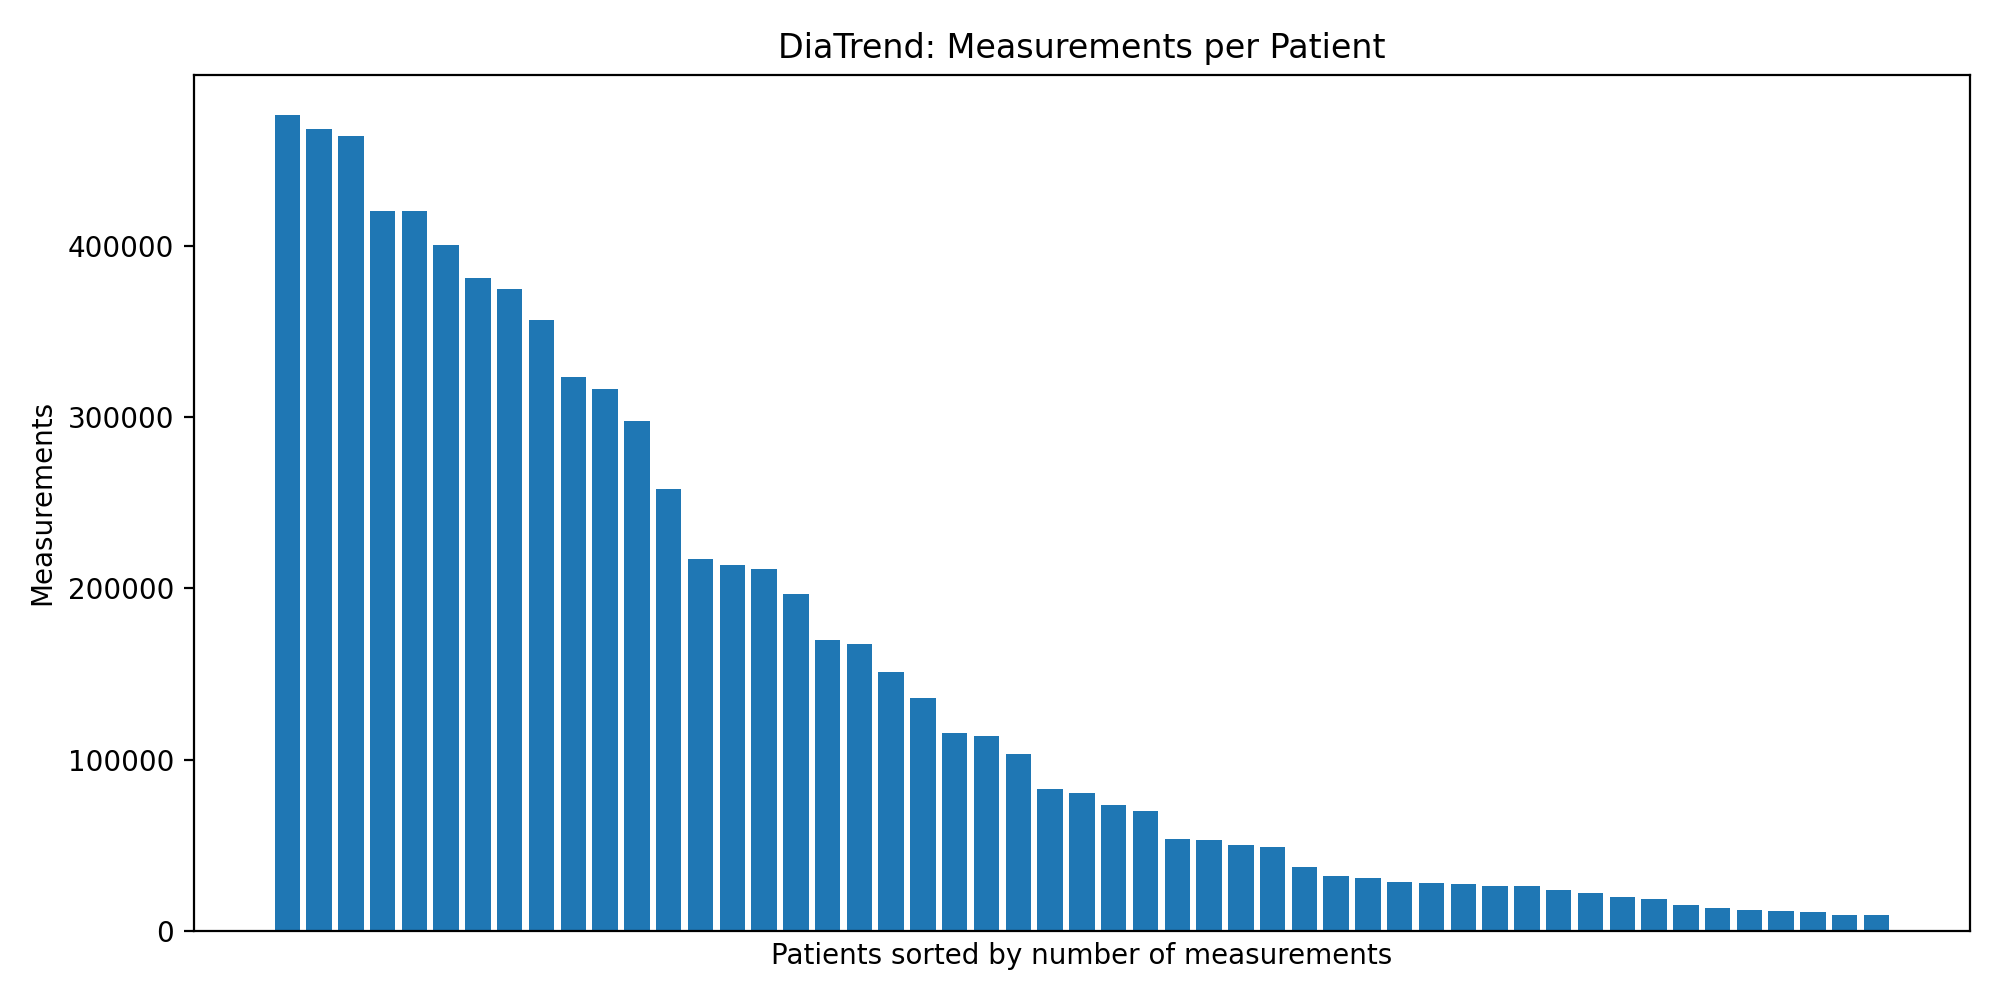
\includegraphics[width=1\textwidth]{images/EDA_Diatrend/measurements_per_patient.png}
    \caption{Measurements per patient in DiaTrend.}
    \label{fig:measurements_per_patients_Diatrend}
\end{figure}

In this dataset, patient contribution to the total glucose measurements distribution is highly uneven, as clearly shown by the descending pattern of Figure~\ref{fig:measurements_per_patients_Diatrend}.

Quantitatively, as shown in Table~\ref{tab:diatrend_patient_contribution}, the largest patient contributes 6.21\% of all measurements, while the top 5 patients account for 29.32\% and the top 10 patients account for 53.27\% of the dataset. In other words, approximately half of all available glucose measurements come from only 10 out of the 51 analyzed patients, which makes the global distribution highly influenced by the glycemic profiles of those individuals with the larger monitoring history. While this finding does not necessarily introduces a bias towards the scope of this thesis -- which is mostly agnostic to individual patient characteristics, it is still relevant enough to be taken into consideration for the subsequent analyses.

\subsection{Glucose Descriptive Statistics}
\label{subsec:diatrend_glucose_statistics}

This section provides a general view of the global distribution of glucose values.

\begin{table}[htbp]
    \centering
    \caption{Glucose descriptive statistics for the DiaTrend dataset.}
    \label{tab:diatrend_glucose_statistics}
    \begin{tabular}{ll}
        \hline
        \textbf{Metric} & \textbf{Value} \\
        \hline
        Minimum glucose & 39 mg/dL \\
        Maximum glucose & 401 mg/dL \\
        Mean glucose & 186.33 mg/dL \\
        Median glucose & 175 mg/dL \\
        Standard deviation & 74.18 mg/dL \\
        \hline
    \end{tabular}
\end{table}

\begin{figure}[htbp]
    \centering
    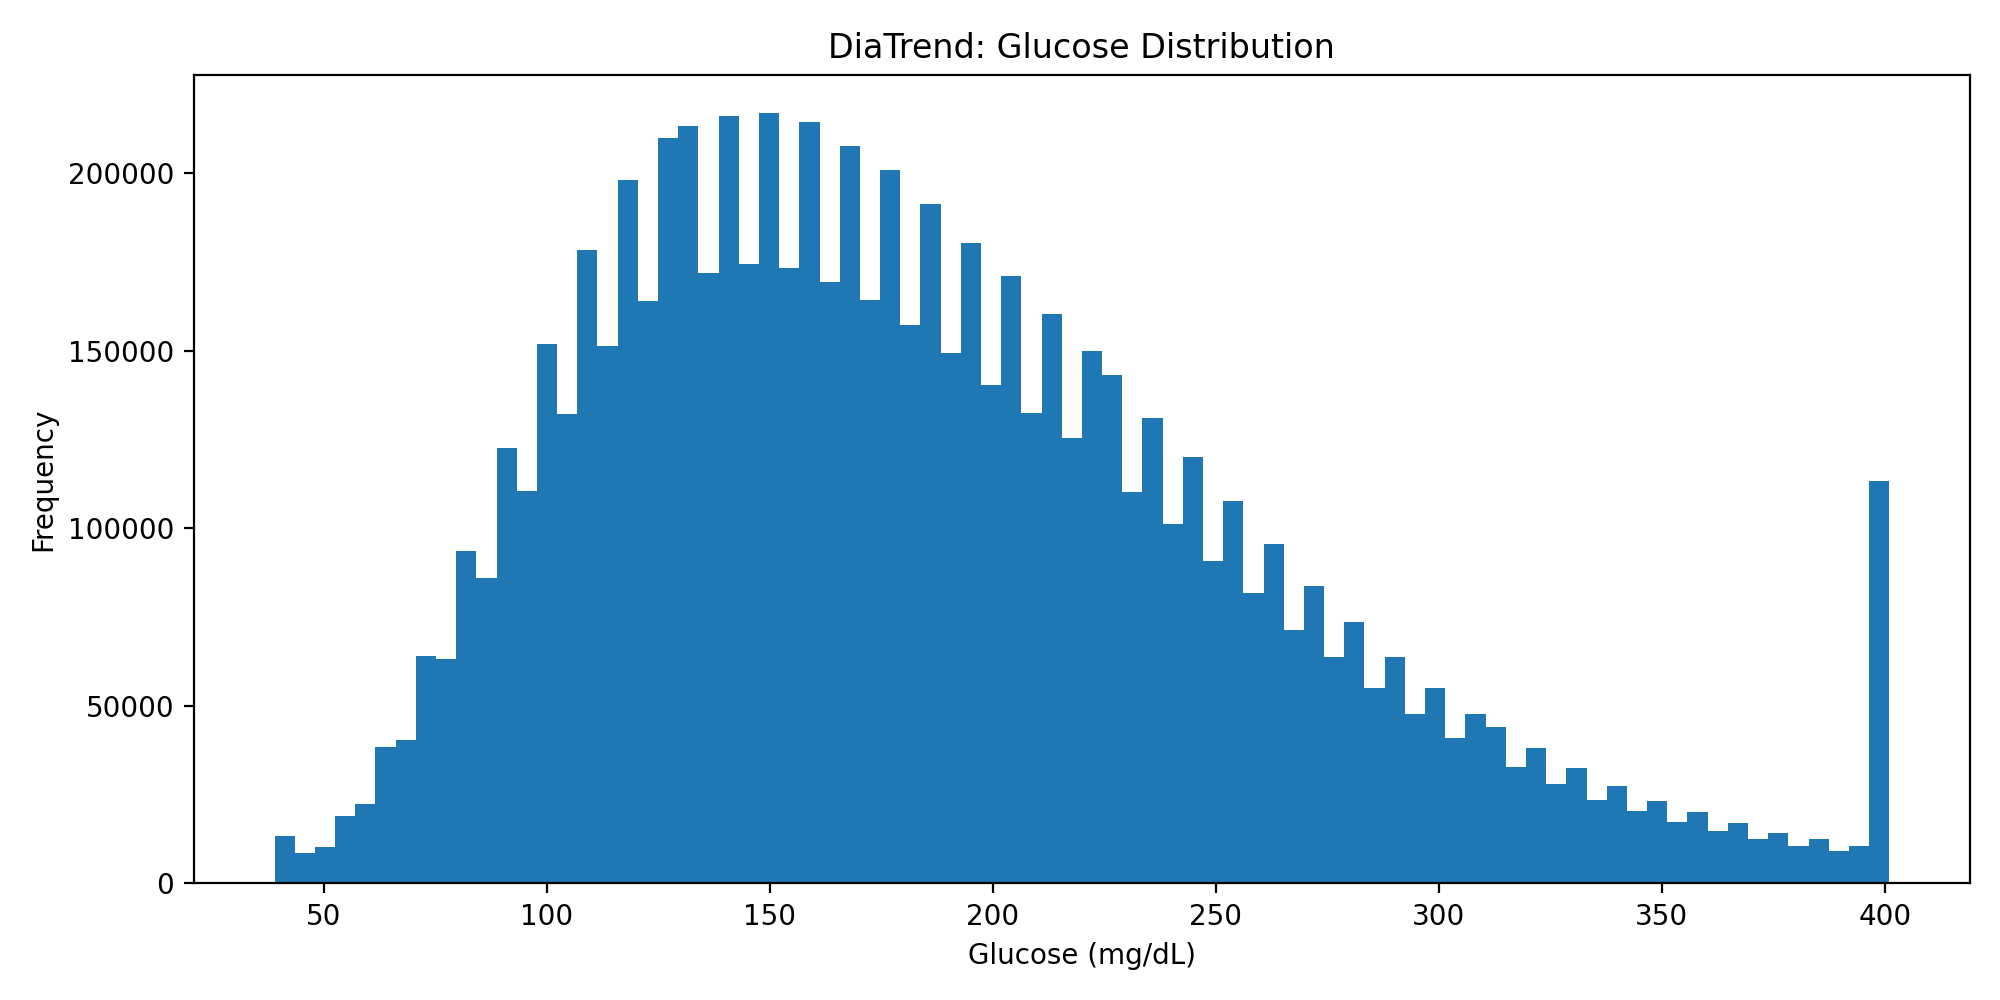
\includegraphics[width=1\textwidth]{images/EDA_Diatrend/glucose_distribution.png}
    \caption{Glucose distribution in DiaTrend.}
    \label{fig:glucose_distribution_Diatrend}
\end{figure}

As shown in Figure~\ref{fig:glucose_distribution_Diatrend}, the glucose distribution follows a typical diabetes-related pattern: the highest concentration of measurements appears around the central normoglycemic and early hyperglycemic regions, while the frequency gradually decreases towards the more extreme hypoglycemic and severe hyperglycemic values.

It is also interesting to note how the histogram presents an irregular pattern with alternating peaks and lower bars. This “one peak, one drop” effect may be related to the measurement resolution, rounding, or preprocessing of CGM values, but it does not change the general shape of the distribution.

\subsection{Glycemic-Range Distribution}
\label{subsec:diatrend_ranges_distribution}

While the previous section describes glucose distribution globally, this one focuses on the analysis of clinically relevant glycemic ranges. As for a reference, the following glycemic ranges are formally presented in Table~\ref{tab:glycemic_range_definitions}:

\begin{table}[htbp]
    \centering
    \caption{Glycemic range definitions.}
    \label{tab:glycemic_range_definitions}
    \begin{tabular}{ll}
        \hline
        \textbf{Glycemic range} & \textbf{Definition} \\
        \hline
        Severe hypoglycemia & $<54$ mg/dL \\
        Hypoglycemia & $54$--$69$ mg/dL \\
        Normoglycemia & $70$--$180$ mg/dL \\
        Hyperglycemia & $181$--$250$ mg/dL \\
        Severe hyperglycemia & $>250$ mg/dL \\
        \hline
    \end{tabular}
\end{table}

The count and the derived percentage of glucose measurements were computed for each of the previous ranges in Diatrend.

\begin{table}[htbp]
    \centering
    \caption{Glycemic range distribution in DiaTrend.}
    \label{tab:diatrend_glycemic_distribution}
    \begin{tabular}{lrr}
        \hline
        \textbf{Glycemic range or category} & \textbf{Count} & \textbf{Percentage} \\
        \hline
        Severe hypoglycemia & 35,291 & 0.46\% \\
        Hypoglycemia & 105,621 & 1.38\% \\
        Normoglycemia & 3,901,129 & 50.88\% \\
        Hyperglycemia & 2,192,705 & 28.60\% \\
        Severe hyperglycemia & 1,432,610 & 18.68\% \\
        \hline
        TBR ($<70$ mg/dL) & 140,912 & 1.84\% \\
        TIR ($70$--$180$ mg/dL) & 3,901,129 & 50.88\% \\
        TAR ($>180$ mg/dL) & 3,625,315 & 47.28\% \\
        \hline
    \end{tabular}
\end{table}

\begin{figure}[htbp]
    \centering
    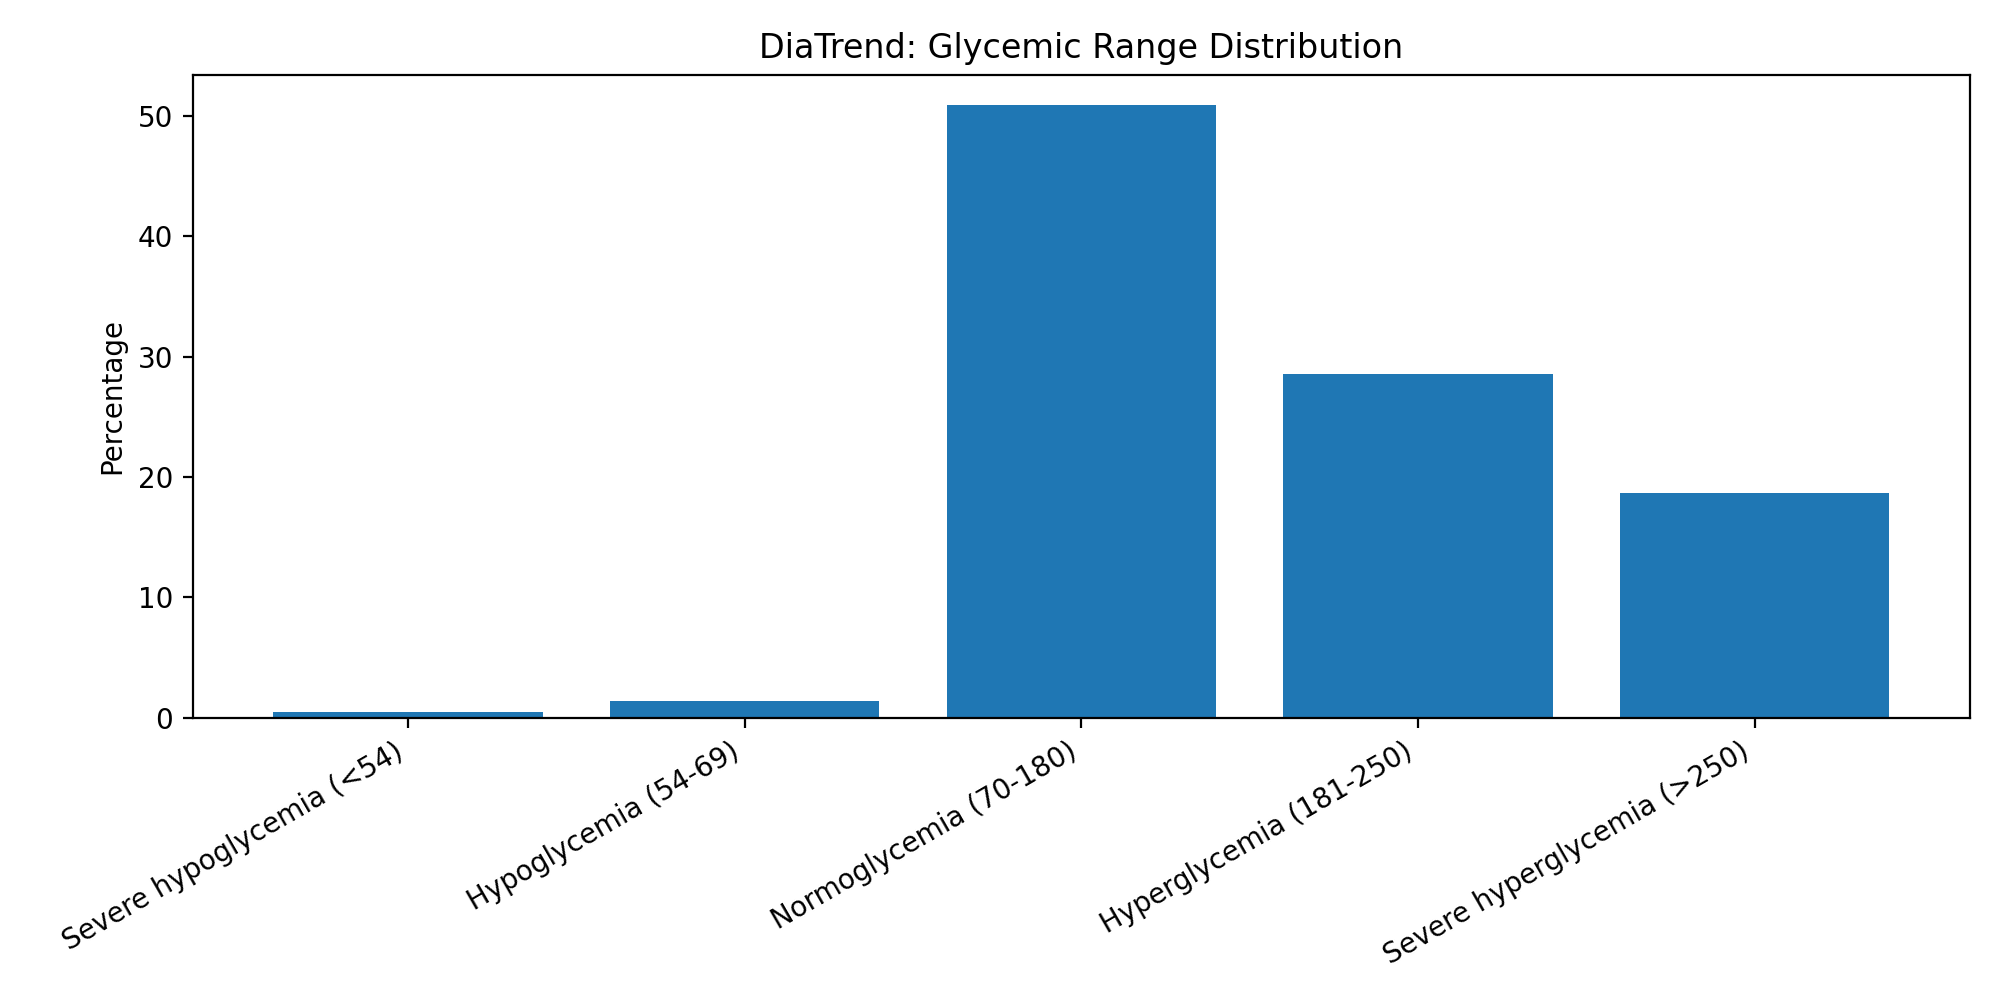
\includegraphics[width=1\textwidth]{images/EDA_Diatrend/glycemic_range_distribution.png}
    \caption{Glycemic range distribution}
    \label{fig:glycemic_range_distribution_Diatrend}
\end{figure}

Figure~\ref{fig:glycemic_range_distribution_Diatrend} makes the imbalance towards clinically critical glycemic ranges clearly visible. Quantitatively, as described in Table~\ref{tab:diatrend_glycemic_distribution}, normo-glycemia is the dominant range representing 50.88\% of all glucose values, hyperglycemia and severe hyperglycemia are also highly represented accounting together for the 47.28\% of the measurements, while hypoglycemia and severe hypoglycemia only account together for the 1.84\% of the total

\begin{table}[htbp]
    \centering
    \caption{Imbalance ratios in DiaTrend.}
    \label{tab:diatrend_imbalance_ratios}
    \begin{tabular}{lr}
        \hline
        \textbf{Ratio} & \textbf{Value} \\
        \hline
        Normoglycemia / hypoglycemia & 27.68 \\
        Normoglycemia / severe hypoglycemia & 110.54 \\
        Normoglycemia / hyperglycemia & 1.78 \\
        Normoglycemia / severe hyperglycemia & 2.72 \\
        Majority range / smallest minority range & 110.54 \\
        \hline
        TIR / TBR & 27.68 \\
        TIR / TAR & 1.08 \\
        \hline
    \end{tabular}
\end{table}

Additionally, the specific imbalance ratios where also quantified in Table~\ref{tab:diatrend_imbalance_ratios}, in order to express the imbalance in more direct quantitative terms, that is: "how much more frequent the majority ranges are compared the clinicall critical ones". For example, in DiaTrend, normoglycemic samples appear 27.68 times more frequently than hypoglycemic samples and 110.54 times more frequently than severe hypoglycemic samples.

\subsection{Patient-Level Glycemic Distribution}
\label{subsec:diatrend_patient_level}

While the global glycemic percentages presented in the previous section are useful, they may hide patient-level differences. For this reason, in order to make a more representative analysis of all the patients, the glycemic ranges distribution was also computed independently for each of them. A summarized version of theses results is presented in Table~\ref{tab:diatrend_patient_glycemic_statistics}

\begin{table}[htbp]
    \centering
    \caption{Patient-level glycemic range statistics in DiaTrend.}
    \label{tab:diatrend_patient_glycemic_statistics}
    \begin{tabular}{lr}
        \hline
        \textbf{Metric} & \textbf{Value} \\
        \hline
        Mean patient TBR & 1.67\% \\
        Median patient TBR & 1.18\% \\
        Minimum patient TBR & 0.06\% \\
        Maximum patient TBR & 9.31\% \\
        \hline
        Mean patient TIR & 53.97\% \\
        Median patient TIR & 52.52\% \\
        Minimum patient TIR & 16.03\% \\
        Maximum patient TIR & 79.57\% \\
        \hline
        Mean patient TAR & 44.36\% \\
        Median patient TAR & 46.50\% \\
        Minimum patient TAR & 18.96\% \\
        Maximum patient TAR & 83.87\% \\
        \hline
    \end{tabular}
\end{table}

\begin{figure}[htbp]
    \centering
    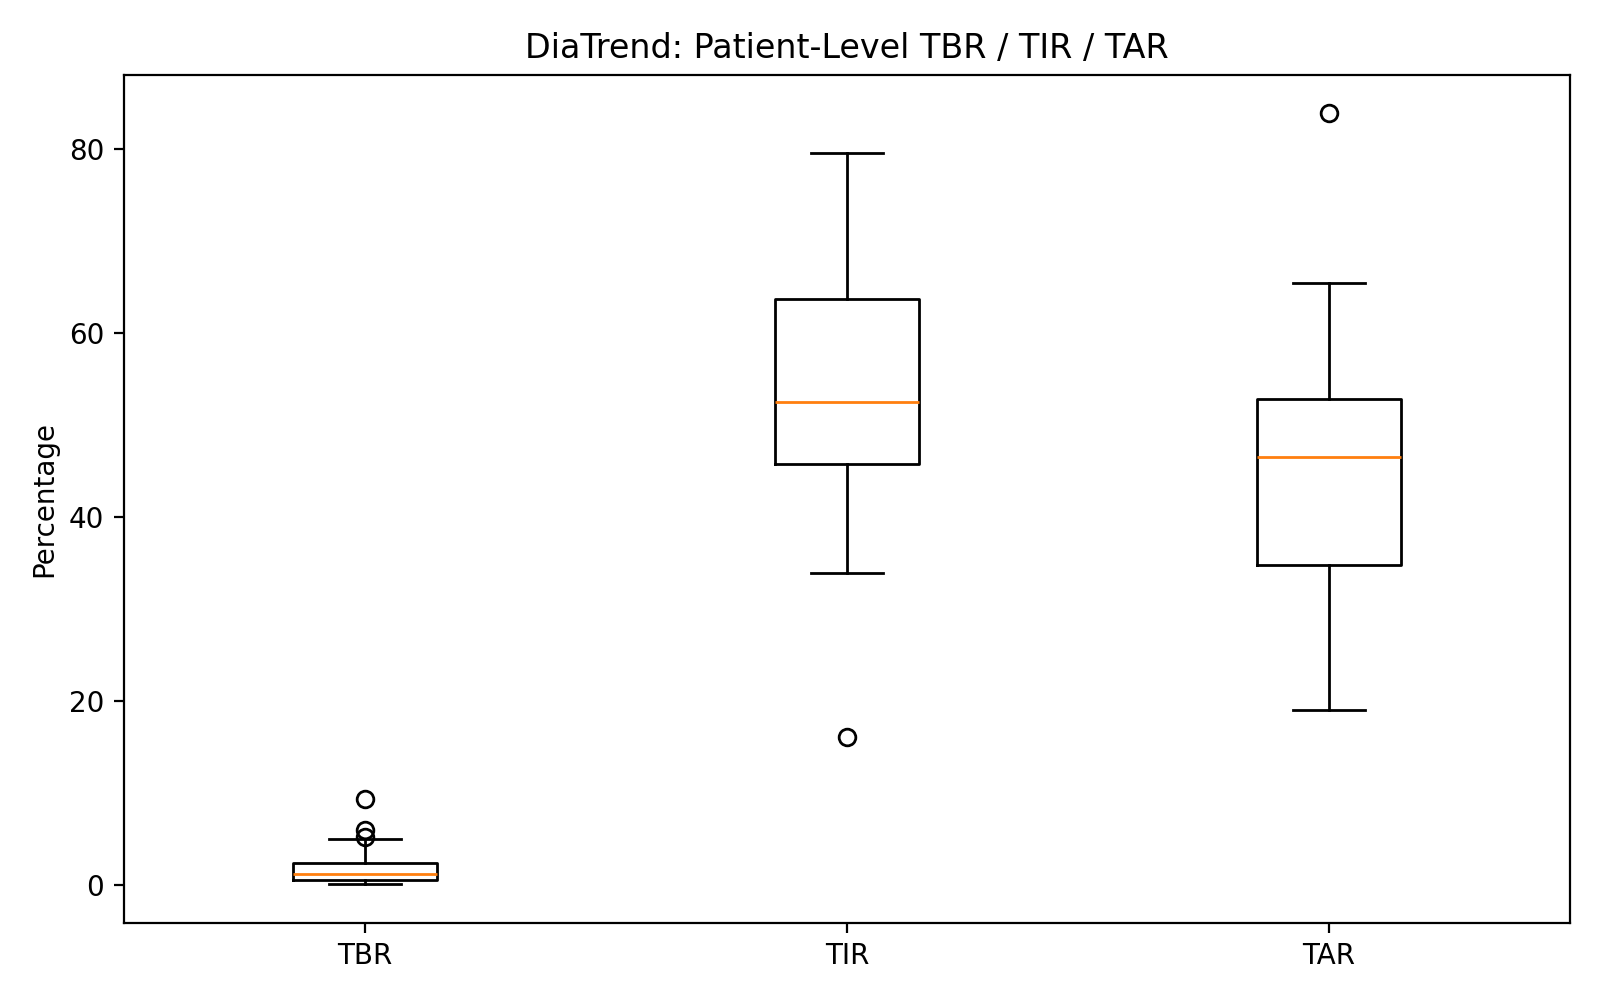
\includegraphics[width=1\textwidth]{images/EDA_Diatrend/patient_level_tbr_tir_tar.png}
    \caption{Glucose distribution in DiaTrend.}
    \label{fig:patient_boxplot_diatrend}
\end{figure}

Figure~\ref{fig:patient_boxplot_diatrend} makes patient-level distribution much more interpretable by presenting it in the form of a box-plot: each box summarises how each of ranges varies for the different patients. This representation allows to interpret whether the imbalance ratios described in general terms are actually equivalent for each patient of the dataset population.

The TBR boxplot is concentrated very close to zero, with a median of 1.18\% and a maximum value of 9.31\%. This indicates that hypoglycemic measurements are mostly consistently rare for most patients, not only at global dataset level. On the contrary, TIR and TAR show much wider variability: TIR has a median of 52.52\%, but ranges from 16.03\% to 79.57\%, while TAR has a median of 46.50\% and ranges from 18.96\% to 83.87\%. Therefore, although TIR is the majority range for 48 out of 51 patients, the balance between normoglycemia and hyperglycemia may vary substantially between different patients. In any case, the plot confirms the consistent under-representation of hypoglycemic values across patients, while normo and hyper-glycemia depends more on the patient.

\subsection{Summary of Findings}
\label{subsec:diatrend_summary}

DiaTrend contains 51 patients and 7,667,356 valid glucose measurements. The dataset covers the period from 2015-12-01 21:01:07 to 2022-06-28 23:59:34, with a total recording span of 2,401 days.

The patient contribution analysis shows that DiaTrend is highly uneven in terms of per-patient measurements availability. The largest patient contributes 6.21\% of all measurements, while the top 10 patients account for 53.27\% of the dataset.

The glucose distribution analysis shows a normo-diabetes pattern: the highest concentration of measurements appears around the central normoglycemic and early hyperglycemic regions, while the frequency gradually decreases towards the more extreme hypoglycemic and severe hyperglycemic values.

The imbalance ratios confirm this pattern quantitatively: normoglycemic samples appear 27.68 times more frequently than hypoglycemic samples and 110.54 times more frequently than severe hypoglycemic samples, while hyperglycemia and severe hyperglycemia appear together globally almost as much as normoglycemia.

At patient level, TBR remains consistently low across patients, which confirms that hypoglycemia is not only globally rare but also generally underrepresented across population. On the other hand, TIR and TAR show wider variability, indicating that the balance between normoglycemia and hyperglycemia highly depends on patient's characteristics.
\section{REPLACE-BG Dataset}
\label{sec:eda_replacebg}

\begin{quote}
\small

\textit{Since the subsequent analyses for REPLACE-BG are analogous to the ones performed for Diatrend, some of the EDA methodology has been omitted.}

\end{quote}

\subsection{Dataset Description}
\label{subsec:replacebg_dataset_description}

Like Diatrend, REPLACE-BG dataset includes both a patient-level information table that provides demographic information, and a glucose measurement table with the timestamped glucose values. Tables' fields are also analogous to those described for Diatrend \ref{subsec:diatrend_dataset_description}. The main descriptive characteristics of the dataset are summarized in Table~\ref{tab:replace_bg_general_description}

\begin{table}[htbp]
    \centering
    \caption{General characteristics of the REPLACE-BG dataset.}
    \label{tab:replace_bg_general_description}
    \begin{tabular}{ll}
        \hline
        \textbf{Metric} & \textbf{Value} \\
        \hline
        Number of patients & 223 \\
        Total number of glucose measurements & 10,432,408 \\
        \hline
        Start date & 2000-01-13 00:01:53 \\
        End date & 2000-11-25 14:39:43 \\
        Total recording span & 317 days \\
        Number of days with measurements & 318 \\
        \hline
        Rows with 5-minute alignment & 11,528,724 \\
        Rows with 15-minute alignment & 3,842,908 \\
        \hline
    \end{tabular}
\end{table}

A consistency check was also performed for REPLACE-BG between the patient metadata table and the measurements table. The metadata file contains information for 223 patients, and all 223 patients are also present in the measurement dataset. Therefore, since no patients appear in one table but not in the other, all subsequent analyses for REPLACE-BG are based on the full set of 223 patients. Table~\ref{tab:replace_bg_general_description} summarises their demographic characteristics.

\begin{table}[htbp]
    \centering
    \caption{Patient information summary for REPLACE-BG.}
    \label{tab:replace_bg_patient_summary}
    \begin{tabular}{lr}
        \hline
        \textbf{Metric} & \textbf{Value} \\
        \hline
        Mean age & 44.17 \\
        Median age & 43 \\
        Minimum age & 19 \\
        Maximum age & 78 \\
        \hline
        Male patients & 111 \\
        Female patients & 112 \\
        \hline
        Mean days with measurements per patient & 173 \\
        Median days with measurements per patient & 178 \\
        \hline
    \end{tabular}
\end{table}

This generic structural description provides the basic context needed for the following analyses.

\subsection{Patient Contribution Analysis}
\label{subsec:replacebg_patient_contribution}

For each patient, the number of glucose measurements and the number of days with at least one measurement were computed, and summarised in Table~\ref{tab:replace_bg_patient_contribution}

\begin{table}[htbp]
    \centering
    \caption{Patient contribution summary in REPLACE-BG.}
    \label{tab:replace_bg_patient_contribution}
    \begin{tabular}{lr}
        \hline
        \textbf{Metric} & \textbf{Value} \\
        \hline
        Mean measurements per patient & 46,782 \\
        Median measurements per patient & 48,688 \\
        Minimum measurements per patient & 10,013 \\
        Maximum measurements per patient & 54,932 \\
        \hline
        Mean days per patient & 173 \\
        Median days per patient & 178 \\
        Minimum days per patient & 38 \\
        Maximum days per patient & 200 \\
        \hline
        Percentage contributed by the largest patient & 0.53\% \\
        Percentage contributed by the top 5 patients & 2.56\% \\
        Percentage contributed by the top 10 patients & 5.08\% \\
        Number of patients contributing 50\% of the dataset & 104 \\
        \hline
    \end{tabular}
\end{table}

\begin{figure}[htbp]
    \centering
    
\includegraphics[width=1\textwidth]{images/EDA_REPLACE/measurements_per_patient.png}
    \caption{Measurements per patient in REPLACE-BG.}
    \label{fig:measurements_per_patients_replace}
\end{figure}

Figure~\ref{fig:measurements_per_patients_replace} shows that REPLACE-BG has a much more homogeneous patient contribution than DiaTrend: bars decrease gradually rather than showing a sharp drop.

Quantitatively, as shown in Table~\ref{tab:replace_bg_patient_contribution}, the largest patient contributes only 0.53\% of all measurements, the top 10 patients contribute 5.08\%, and 104 out of the 223 patients are required to account for 50\% of the dataset. Compared with DiaTrend, where the top 10 patients accounted for more than half of all measurements, REPLACE-BG is much less dominated by a small subset of individuals. Therefore, from a patient-contribution perspective, REPLACE-BG is much more balanced.

\subsection{Glucose Descriptive Statistics}
\label{subsec:replacebg_glucose_statistics}

The global distribution of glucose values was also analyzed and summarised in Table~\ref{tab:replace_bg_glucose_statistics}.

\begin{table}[htbp]
    \centering
    \caption{Glucose descriptive statistics in REPLACE-BG.}
    \label{tab:replace_bg_glucose_statistics}
    \begin{tabular}{lr}
        \hline
        \textbf{Metric} & \textbf{Value} \\
        \hline
        Minimum glucose & 39 mg/dL \\
        Maximum glucose & 401 mg/dL \\
        Mean glucose & 159.89 mg/dL \\
        Median glucose & 150 mg/dL \\
        Standard deviation & 64.13 mg/dL \\
        \hline
    \end{tabular}
\end{table}

\begin{figure}[htbp]
    \centering
    
\includegraphics[width=1\textwidth]{images/EDA_REPLACE/glucose_distribution.png}
    \caption{Glucose distribution in REPLACE-BG.}
    \label{fig:glucose_distribution_replace}
\end{figure}

As shown in Figure~\ref{fig:glucose_distribution_replace}, the glucose distribution follows a typical diabetes-related pattern: the highest concentration of measurements appears around the central normoglycemic and early hyperglycemic regions, while the frequency gradually decreases towards the more extreme hypoglycemic and severe hyperglycemic values.

The histogram also presents an irregular “one peak, one drop” pattern, that may be related to the measurement resolution. However, it does not change the general shape of the distribution.

\subsection{Glycemic-Range Distribution}
\label{subsec:replacebg_ranges_distribution}

As the central part of the EDA for this thesis, glycemic ranges distribution of REPLACE-BG dataset was also studied. As for a reference, the same ranges defined in Table~\ref{tab:glycemic_range_definitions} are used. Results are presented summarised in Table~\ref{tab:replace_bg_glycemic_distribution}

\begin{table}[htbp]
    \centering
    \caption{Glycemic range distribution in REPLACE-BG.}
    \label{tab:replace_bg_glycemic_distribution}
    \begin{tabular}{lrr}
        \hline
        \textbf{Glycemic range or category} & \textbf{Count} & \textbf{Percentage} \\
        \hline
        Severe hypoglycemia & 94,499 & 0.91\% \\
        Hypoglycemia & 291,856 & 2.80\% \\
        Normoglycemia & 6,636,660 & 63.62\% \\
        Hyperglycemia & 2,437,218 & 23.36\% \\
        Severe hyperglycemia & 972,175 & 9.32\% \\
        \hline
        TBR ($<70$ mg/dL) & 386,355 & 3.70\% \\
        TIR ($70$--$180$ mg/dL) & 6,636,660 & 63.62\% \\
        TAR ($>180$ mg/dL) & 3,409,393 & 32.68\% \\
        \hline
    \end{tabular}
\end{table}

\begin{figure}[htbp]
    \centering
    
\includegraphics[width=1\textwidth]{images/EDA_REPLACE/glycemic_range_distribution.png}
    \caption{Glycemic range distribution}
    \label{fig:glycemic_range_distribution_replace}
\end{figure}

Figure~\ref{fig:glycemic_range_distribution_replace} makes the imbalance towards clinically critical glycemic ranges clearly visible. Quantitatively, as described in Table~\ref{tab:replace_bg_glycemic_distribution}, normo-glycemia is the dominant range representing 63.62\% of all valid glucose measurements, hyperglycemia and severe hyperglycemia are also very present -- with TAR accounting for 32.68\% of the measurements, while hypoglycemic ranges are much smaller in the graph, accounting for 3.70\% of the total. This graph then provides visual confirmation of the under-representation of hypoglycemic regions compared with normoglycemia and hyperglycemia.

\begin{table}[htbp]
    \centering
    \caption{Imbalance ratios in REPLACE-BG.}
    \label{tab:replace_bg_imbalance_ratios}
    \begin{tabular}{lr}
        \hline
        \textbf{Ratio} & \textbf{Value} \\
        \hline
        Normoglycemia / hypoglycemia & 17.18 \\
        Normoglycemia / severe hypoglycemia & 70.23 \\
        Normoglycemia / hyperglycemia & 2.72 \\
        Normoglycemia / severe hyperglycemia & 6.83 \\
        Majority range / smallest minority range & 70.23 \\
        \hline
        TIR / TBR & 17.18 \\
        TIR / TAR & 1.95 \\
        \hline
    \end{tabular}
\end{table}

Moreover, the concrete imbalance ratios where also quantified in Table~\ref{tab:replace_bg_imbalance_ratios}. For example normoglycemic samples appear 17.18 times more frequently than hypoglycemic samples and 70.23 times more frequently than severe hypoglycemic samples.

\subsection{Patient-Level Glycemic Distribution}
\label{subsec:replacebg_patient_level}

The glycemic ranges distribution was also computed independently for each patient in order to make a more horizontally representative analysis. A summarized version of the results is presented in Table~\ref{tab:replace_bg_patient_glycemic_statistics}

\begin{table}[htbp]
    \centering
    \caption{Patient-level glycemic range statistics in REPLACE-BG.}
    \label{tab:replace_bg_patient_glycemic_statistics}
    \begin{tabular}{lr}
        \hline
        \textbf{Metric} & \textbf{Value} \\
        \hline
        Mean patient TBR & 3.70\% \\
        Median patient TBR & 3.24\% \\
        Minimum patient TBR & 0.01\% \\
        Maximum patient TBR & 14.20\% \\
        \hline
        Mean patient TIR & 63.37\% \\
        Median patient TIR & 63.18\% \\
        Minimum patient TIR & 16.94\% \\
        Maximum patient TIR & 96.77\% \\
        \hline
        Mean patient TAR & 32.94\% \\
        Median patient TAR & 33.91\% \\
        Minimum patient TAR & 0.51\% \\
        Maximum patient TAR & 82.00\% \\
        \hline
    \end{tabular}
\end{table}

\begin{figure}[htbp]
    \centering
    
\includegraphics[width=1\textwidth]{images/EDA_REPLACE/patient_level_tbr_tir_tar.png}
    \caption{Glucose distribution in REPLACE-BG.}
    \label{fig:patient_boxplot_replace}
\end{figure}

Patient-level variabilitiy is also presented in the form of a box-plot in Figure~\ref{fig:patient_boxplot_replace}.

TBR boxplot is also concentrated very close to zero, with a median of 3.24\% and a maximum value of 14.20\%. This indicates that hypoglycemic measurements are mostly consistently rare for most patients. On the other hand, TIR and TAR show much wider variability: TIR has a median of 63.18\%, but ranges from 16.94\% to 96.77\%, while TAR has a median of 33.91\% and ranges from 0.51\% to 82\%. In any case, the plot confirms the consistent under-representation of hypoglycemic values across patients in this dataset too.

In this case, it is important to highlight the substantial degree of variability between patients, especially for TIR and TAR. The wide spread of the boxplots and the presence of several outliers indicate that, although normoglycemia is still the dominant range for most individuals, the proportion of time spent in range or above range differs considerably across the population. In practical terms, this means that REPLACE-BG shows a consistent global imbalance against hypoglycemia, but patient glycemic profiles present a high degree of  heterogeneity with respect to TIR and TAR.

\subsection{Summary of Findings}
\label{subsec:replacebg_summary}

REPLACE-BG contains 223 patients and 10,432,408 valid glucose measurements. The dataset covers the period from 2000-01-13 00:01:53 to 2000-11-25 14:39:43, with a total recording span of 317 days.

It shows a very homogeneous patient contribution: the largest patient contributes only 0.53\% of all measurements, the top 10 patients account only for 5.08\% of the total, and 104 out of 223 patients are required to accumulate 50\% of the dataset. This indicates that the global glucose distribution is less likely to be dominated by a small subset of patients.

The glucose distribution analysis shows a normo-diabetes pattern.

The imbalance ratios quantitatively connfirms the glycemic ranges imbalance. They show that normoglycemic samples appear 17.18 times more frequently than hypoglycemic samples and 70.23 times more frequently than severe hypoglycemic samples.

At patient level, as expected, TBR remains consistently low across patients. However, it is important to highlight the substantial variability across patients population in TIR and TAR: the minimum and maximum in both ranges can differ up to 80\% from one patient to another.
\input{chapters/03_T1Diabetes}

\section{Cross-Dataset Comparison}
\label{sec:eda_cross_dataset_comparison}
With all the three datasets analyzed separately, this section cross-compares them with each other, in order to determine whether glycemic ranges imbalance is consistent across the three of them, and to what extent.

\begin{table}[htbp]
    \centering
    \caption{General comparison of the three datasets.}
    \label{tab:general_dataset_comparison}

    \setlength{\tabcolsep}{5pt}
    \renewcommand{\arraystretch}{1.15}

    \begin{tabularx}{\textwidth}{Xccc}
        \hline
        \textbf{Metric}
        & \textbf{DiaTrend}
        & \textbf{REPLACE-BG}
        & \textbf{\shortstack{T1Diabetes\\Granada}} \\
        \hline

        Number of patients
        & 51
        & 223
        & 643 \\

        Number of valid glucose measurements
        & 7,667,356
        & 10,432,408
        & 22,233,264 \\

        Recording span
        & 2,401 days
        & 317 days
        & 1,535 days \\

        Mean measurements per patient
        & 150,340
        & 46,782
        & 34,577 \\

        Median measurements per patient
        & 80,488
        & 48,688
        & 28,223 \\

        Patients contributing 50\% of the dataset
        & 10
        & 104
        & 158 \\

        \hline
    \end{tabularx}
\end{table}

As shown in Table~\ref{tab:general_dataset_comparison}, the three datasets strongly differ on the number of patients, duration, and patient contribution. T1DiabetesGranada is the largest dataset in both number of patients and number of valid glucose measurements. REPLACE-BG has the most homogeneous per-patient contribution compared to the others. And DiaTrend, despite having the smallest number of patients, has the longest recording span, and as a result the highest mean number of measurements per patient.

Therefore, the most important difference appears in per-patient contribution. Both DiaTrend and T1Diabetes are relatively concentrated in a small subset of patients, since approximately only 19\% and 26\%, respectively, of the patients contribute 50\% of the corresponding dataset. In contrast, REPLACE-BG requires approximately 46\% of the patients to reach 50\% of the measurements.

\begin{table}[htbp]
    \centering
    \caption{Cross-dataset comparison of glycemic ranges.}
    \label{tab:cross_dataset_glycemic_comparison}
    \begin{tabular}{lrrr}
        \hline
        \textbf{Metric} & \textbf{DiaTrend} & \textbf{REPLACE-BG} & \textbf{T1DiabetesGranada} \\
        \hline
        Severe hypoglycemia & 0.46\% & 0.91\% & 0.99\% \\
        Hypoglycemia & 1.38\% & 2.80\% & 3.78\% \\
        Normoglycemia & 50.88\% & 63.62\% & 59.70\% \\
        Hyperglycemia & 28.60\% & 23.36\% & 23.76\% \\
        Severe hyperglycemia & 18.68\% & 9.32\% & 11.77\% \\
        \hline
        TBR & 1.84\% & 3.70\% & 4.77\% \\
        TIR & 50.88\% & 63.62\% & 59.70\% \\
        TAR & 47.28\% & 32.68\% & 35.52\% \\
        \hline
    \end{tabular}
\end{table}

Table~\ref{tab:cross_dataset_glycemic_comparison} confirms that the dominance of each of the 5 clinical glycemic ranges with respect to the others is repeated across the three datasets. Normoglycemia is always the majority range. TAR is also very present, although not as much as TIR. And TBR is consistently underrepresented in all datasets, with severe hypoglycemia also being the smallest glycemic range in all three datasets, remaining below 1\% in all of them.

However, the strength of that dominance varies from one dataset to the other. REPLACE-BG has the highest TIR percentage, with 63.62\% of its measurements in range, followed by T1DiabetesGranada with 59.70\% and DiaTrend with 50.88\%. TBR is lowest in DiaTrend, where it represents only 1.84\% of measurements, followed by REPLACE-BG with 3.70\% and T1DiabetesGranada with 4.77\%. The main difference between datasets appears in the hyperglycemic region. DiaTrend has the highest TAR percentage, with 47.28\% of measurements above 180 mg/dL, including 18.68\% in severe hyperglycemia. while REPLACE-BG and T1DiabetesGranada show lower TAR percentages.

An additional assessment of this imbalance is presented in Table~\ref{tab:cross_dataset_imbalance_comparison} with the imbalance ratios of each dataset

\begin{table}[htbp]
    \centering
    \caption{Cross-dataset comparison of imbalance ratios.}
    \label{tab:cross_dataset_imbalance_comparison}
    \begin{tabular}{lrrr}
        \hline
        \textbf{Ratio} & \textbf{DiaTrend} & \textbf{REPLACE-BG} & \textbf{T1DiabetesGranada} \\
        \hline
        Normo / hypo & 27.68 & 17.18 & 12.51 \\
        Normo / severe hypo & 110.54 & 70.23 & 60.17 \\
        Normo / hyper & 1.78 & 2.72 & 2.51 \\
        Normo / severe hyper & 2.72 & 6.83 & 5.07 \\
        Majority / minority & 110.54 & 70.23 & 60.17 \\
        \hline
        TIR / TBR & 27.68 & 17.18 & 12.51 \\
        TIR / TAR & 1.08 & 1.95 & 1.68 \\
        \hline
    \end{tabular}
\end{table}

These results show that the imbalance problem is not symmetric: low-glucose values, especially severe hypoglycemia, are consistently rare across all datasets, whereas high-glucose values are also less frequent than normoglycemia but present in higher proportions than low ones.

\begin{table}[htbp]
    \centering
    \caption{Cross-dataset comparison of patient-level variability.}
    \label{tab:cross_dataset_patient_variability}
    \small
    \setlength{\tabcolsep}{4pt}
    \begin{tabularx}{\textwidth}{Xrrr}
        \hline
        \textbf{Metric} &
        \textbf{DiaTrend} &
        \textbf{REPLACE-BG} &
        \textbf{T1DiabetesGranada} \\
        \hline
        Mean patient TBR & 1.67\% & 3.70\% & 4.45\% \\
        Median patient TBR & 1.18\% & 3.24\% & 3.32\% \\
        Mean patient TIR & 53.97\% & 63.37\% & 59.25\% \\
        Median patient TIR & 52.52\% & 63.18\% & 60.05\% \\
        Mean patient TAR & 44.36\% & 32.94\% & 36.30\% \\
        Median patient TAR & 46.50\% & 33.91\% & 35.14\% \\
        \hline
        Patients with zero hypoglycemia & 0 & 0 & 2 \\
        Patients with zero severe hypoglycemia & 1 & 1 & 27 \\
        Patients with zero severe hyperglycemia & 0 & 0 & 3 \\
        \hline
        Patients where TIR is the majority range & 48 & 219 & 608 \\
        Patients where TIR is the majority range (\%) &
        94.12\% & 98.21\% & 94.56\% \\
        \hline
    \end{tabularx}
\end{table}

The patient-level comparison presented in Table~\ref{tab:cross_dataset_patient_variability} confirms that the imbalance patterns found globally are also largely present across individual patients and are not caused by asymmetric contributions from patients with different glycemic profiles. Across the three datasets, TBR generally remains low at the patient level, TIR is the majority range for most patients, and TAR represents a substantial but more variable proportion of measurements. Therefore, the dominance of normoglycemia and the underrepresentation of hypoglycemia are not driven by only a few large contributors but are broadly present at the patient level.

However, this is to be considered a general pattern, and does not necessarily imply that minority glycemic ranges are represented uniformly across every single individual. This is particularly evident in T1DiabetesGranada, where some patients contain no measurements in the hypoglycemic, severe hypoglycemic, or severe hyperglycemic ranges. Therefore, although the global and per-patient imbalance patterns mostly support the use of a common balancing strategy, the methodology should still remain sensitive to dataset-specific distributions and patient-level differences.

In summary, the comparison shows a consistent pattern across the three datasets: normoglycemia is the majority range, hypoglycemia is the clearest minority region, and severe hyperglycemia is underrepresented but less rare than hypoglycemia; which is also mostly present at patient-level.

\section{Summary and Implications for Data Balancing}
\label{sec:eda_summary}

This chapter explored the structure and glucose distributions of DiaTrend, REPLACE-BG, and T1DiabetesGranada, in order the quantify the imbalance across clinically relevant glycemic ranges.

The results show that normoglycemia is the majority range in all three datasets. TIR represents 50.88\% of DiaTrend, 63.62\% of REPLACE-BG, and 59.70\% of T1DiabetesGranada. 

On the contrary, hypoglycemia is consistently the most underrepresented clinically relevant region. TBR represents only 1.84\% of DiaTrend, 3.70\% of REPLACE-BG, and 4.77\% of T1DiabetesGranada. Severe hypoglycemia is even rarer, remaining below 1\% in all datasets.

Severe hyperglycemia is also less frequent than normoglycemia in all datasets, but it is not as rare as hypoglycemia. It represents 18.68\% of DiaTrend, 9.32\% of REPLACE-BG, and 11.77\% of T1DiabetesGranada. This means that severe hyperglycemia should still be considered a minority region, but the imbalance against it is less extreme than the imbalance against hypoglycemia.

Therefore, although the exact proportion differs between datasets, the same general pattern is observed globally: most glucose measurements are concentrated in the normoglycemic range, low-glucose values are the clearest minority region, and and hyperglycemia is also less represented than normoglycemia, but not as rare as hypoglycemia.

The patient-level analysis shows that, although the specific values for each patient have some natural degree of variability, the patterns found globally are also analogously present across population. TIR is the majority range for 94.12\% of DiaTrend patients, 98.21\% of REPLACE-BG patients, and 94.56\% of T1DiabetesGranada patients. At the same time, the representation of minority ranges varies across individuals, especially in T1DiabetesGranada, where some patients have no measurements in specific minority glycemic ranges.

These findings have direct implications for data balancing. First, a balancing strategy is clearly justified to be approachable because all three datasets clearly show the expected glycemic-range imbalance. Second, hypoglycemia, severe hypoglycemia and severe hyperglycemia should recieve particular attention in the balancing methodology, given their consistent rarity -- although different from each other -- and clinical importance. Finally, the methodology should not only be global, but also patient-aware: it should preserve individual patient distributions and glycemic profiles, and avoid generating samples for absent ranges.

In summary, the EDA confirms that the selected datasets are suitable for studying glycemic-range imbalance in T1D CGM prediction. The observed imbalance is not merely theoretical, but empirically present across all three datasets, both globally and a patient level. The graphical and quantitative results provide the basis for defining the data balancing methodology in the next chapter, with the objective to increase the representation of clinically critical minority glucose regions without unnecessarily distorting the patient-level structure of the original data.